%%%%%%%%%%%%%%%%%%%%%%%%%%%%%%%%%%%%%%%%%%%%%%%%%%%%%%%%%%%%%%%%%%%
\section{Mémoire virtuelle} \label{sec:memoire_virtuelle}
%%%%%%%%%%%%%%%%%%%%%%%%%%%%%%%%%%%%%%%%%%%%%%%%%%%%%%%%%%%%%%%%%%%


%%%%%%%%%%%%%%%%%%%%%%%%%%%%%%%%%%%%%%%%%%%%%%%%%%%%%%%%%%%%%%%%%%%
\subsection{Contexte et historique de la gestion mémoire}
%%%%%%%%%%%%%%%%%%%%%%%%%%%%%%%%%%%%%%%%%%%%%%%%%%%%%%%%%%%%%%%%%%%

La mémoire est une des ressources les plus importantes des architectures modernes. Sa gestion doit être la plus performante possible  si l'on souhaite minimser au maximum le trou de performance séparant les mémoires et les processeurs. Si la hiérarchie de mémoire est la réponse matérielle à ce challenge la mémoire virtuelle est une réponse logicielle. Avant de la présenter en détail, cette introduction à pour but de motiver son utilité.

\subsubsection{Utilité de l'abstraction de la mémoire}
%%%%%%%%%%%%%%%%%%%%%%%%

Sans abstraction mémoire, tous les programmes et le système d'exploitation partagerai le même espace d'adressage. Cette implémentation, utilisée par les premières architectures, a deux inconvénients majeurs. Le premier concerne la sécurité de l'exécution d'un programme. S'il venait à écrire dans une zone mémoire réservée au système d'exploitation, un arrêt brutal du système pourrait survenir. De plus, lors de l'exécution de plusieurs processus sur le même processeur, deux programmes différents pourraient accéder et/ou modifier des données ne lui appartenant pas. Une solution pour contourner ce problème est d'alterner l'exécution de chaque processus en vidant et chargeant ses données depuis le stockage, engendrant le deuxième inconvénient d'un système sans abstraction mémoire: la performance. Bien que des threads puisse tout de même être utilisés (ils appartiennent au même processus et ont accès au même espace mémoire) l'utilisation de cette architecture serait très impactée. Par exemple, un utilisateur ne pourrait pas avoir plusieurs fenêtre exécutant des programmes différents en parallèle. L'utilisation de serveurs multi-utilisateurs ne serait alors même pas envisageable. L'absence d'abstraction mémoire, ou adresse direct, ne trouve d'application aujourd'hui que dans les systèmes embarqués. Le constructeur du système est généralement le seul utilisateur du processeur et est donc maître de son utilisation et peut réaliser des allocations mémoires manuellement.

\paragraph{L'abstraction par réallocation statique} a été implémentée sur l'ordinateur IBM 260 en 1965 \cite{Britannica} pour permettre l'exécution simultanée de plusieurs processus. Le système d'exploitation alloue une adresse de base à chaque processus. Lorsqu'une processus réalise un accès mémoire, un matériel s'occupait de décaler tous ses accès mémoires à partir de l'adresse de base. Ce mécanisme, invisible pour le programmeur était fonctionnelle mais impactait les performances du programme. Elle pouvait s'avérer complexe à mettre en place car il fallait distinguer les adresses à convertir et celle ne le nécessitant pas (un saut en mémoire par exemple).

\paragraph{L'abstraction de l'espace d'adressage} permet de donner son propre espace d'adresses à chaque processus indépendant les uns des autres. L'allocation dynamique permet de mapper l'espace mémoire d'un processus à un espace physique de la mémoire en utilisant deux registres \textit{base} et \textit{limite} comme sur le processeur Intel  8088. La méthode de \textit{va-et-vient} ou \textit{swapping} peut être utilisée pour gérer les déplacements des processus entre la mémoire et le stockage. Cette méthode est illustrée dans la \autoref{pic:memory_swapping}. L'inconvénient de cette méthode est la création de trous dans la mémoire, empêchant son utilisation optimale.  Des techniques de compactage ont été alors élaborées, mais était souvent très coûteuses (5s pour compacter 1GB de mémoire \cite{tanenbaum2008systeme}). De plus cette méthode ne permet pas de gérer les grands logiciels dont la taille ne permet pas d'être stockés en intégralité. Bien que des techniques utilisant les segments de recouvrement (\textit{overlays}) \cite{sherman1992method} aient permis  d'adapter le \textit{va-et-vient} a ces grand processus, la technique adoptée depuis est connue sous le terme de \textit{mémoire virtuelle}.


\begin{figure}
    \center
    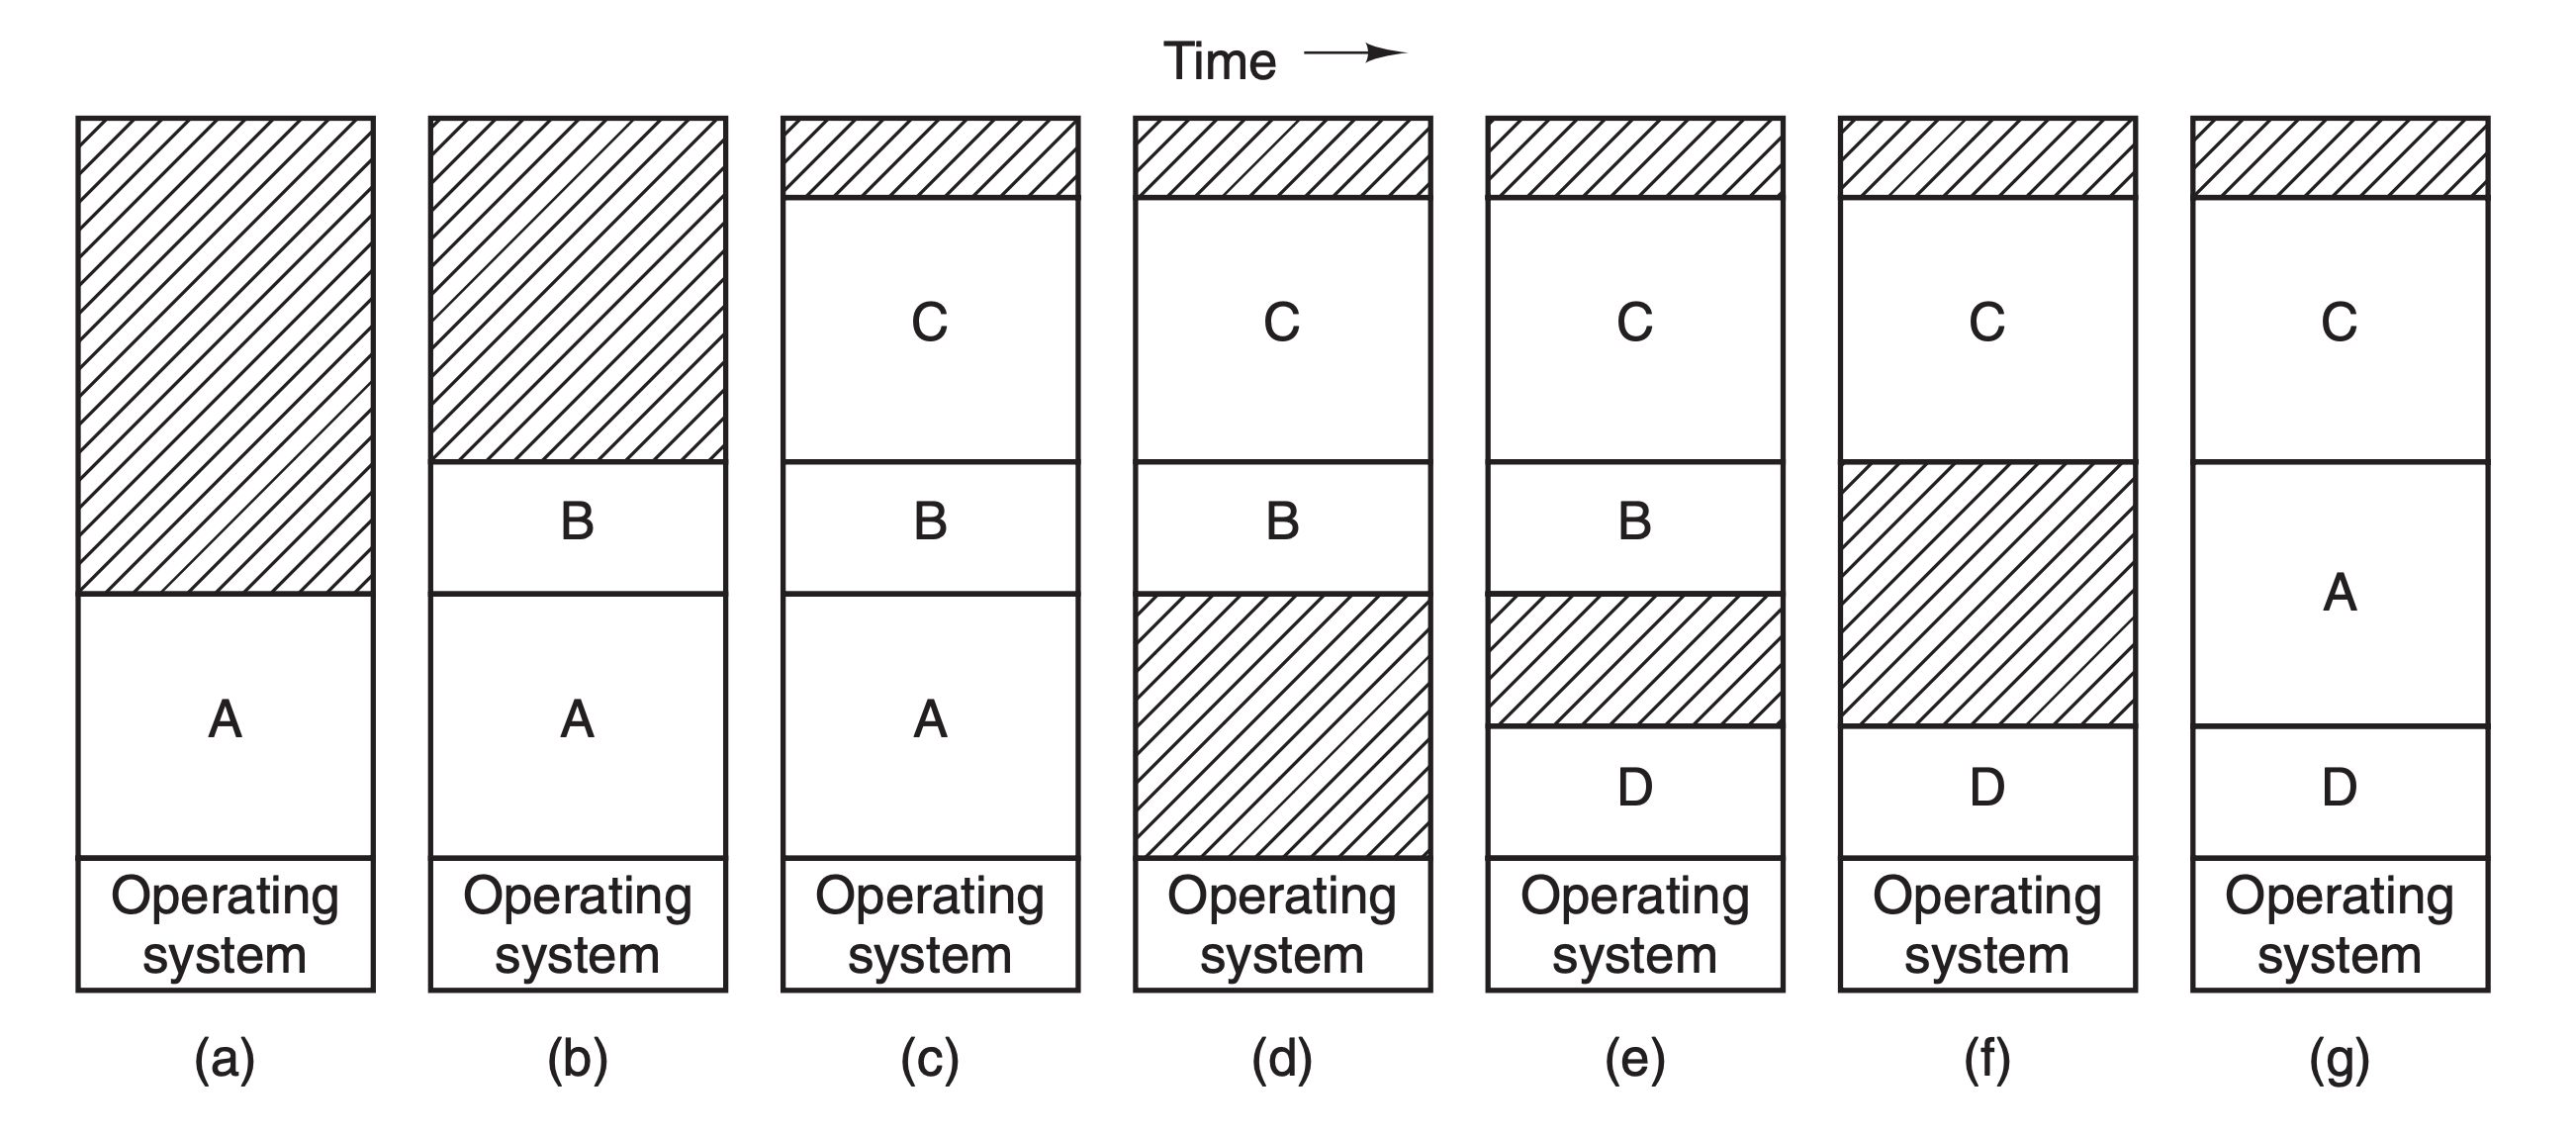
\includegraphics[width=10cm]{images/memory_swapping.png}
    \caption{\label{pic:memory_swapping} Technique de va-et-vient pour gérer la mémoire dynamiquement. Les processus A, B, et C sont créés dans les étapes (a), (b) et (c). Lors de la création d'un processus D à l'étape (d), le système d'exploitation doit enlever un processus de la mémoire pour lui faire de la place. Lors de l'étape (f) et (g), le processus B laisse sa place pour que A puisse continuer son exécution. Entre l'étape (c) et (g) le processus A est exécuté à partir de deux espace d'adressage physique différents (graphique extrait de \cite{tanenbaum2008systeme})}.
\end{figure}





%%%%%%%%%%%%%%%%%%%%%%%%%%%%%%%%%%%%%%%%%%%%%%%%%%%%%%%%%%%%%%%%%%%
\subsection{La pagination}
%%%%%%%%%%%%%%%%%%%%%%%%%%%%%%%%%%%%%%%%%%%%%%%%%%%%%%%%%%%%%%%%%%%


\subsubsection{Motivations}
%%%%%%%%%%%%%%%%%%%%%%%%
La mémoire virtuelle a été implémentée pour gérer de façon efficace des processus dont la taille est plus grande que l'espace mémoire disponible. L'optimisation par \textit{overlay} présentée précédemment était très compliqué à mettre en oeuvre et devait être réalisée par le programmeur. La seconde motivation était de gérer efficacement la mémoire la somme des tailles des processus exécutés dépasse l'espace mémoire disponible. En d'autre terme, il fallait un mécanisme permettant l'exécution d'une programme sans qu'il soit chargé en totalité en mémoire. La solution devait aussi permettre de gérer facilement les changements de taille des processus de façon efficace, sans avoir à recopier la totalité du programme lors d'une allocation mémoire (\textit{malloc)}. Enfin, la mémoire virtuelle doit assurer la sécurité de l'exécution de plusieurs programme sur une même architecture en évitant les bugs et les vols de données.


\subsubsection{Les pages}
%%%%%%%%%%%%%%%%%%%%%%%%
Le principe de la mémoire virtuelle repose sur le principe de donner à chaque processus sont propre espace d'adressage mémoire. Chaque processus peut travailler sur l'adresse \textit{0x100}, car en réalité le mécanisme de mémoire virtuelle fait correspondre cette \textbf{adresse virtuelle} à différentes \textbf{adresse physique}. Pour cela, son \textbf{espace d'adressage virtuelle} est découpé en petites entités appelées \textbf{pages} qui contiennent un \textbf{espace d'adressage physique} contiguës. Chaque page est \textit{mappée} sur des adresses physiques (aussi contiguës) formant un \textbf{cadre de page} (\textit{page frame}). Une page et son cadre de page associé contiennent le même nombre d'adresses. Deux pages contiguës ne correspondent pas forcément à deux cadres de pages contiguës. Les pages et les cadres de pages ont la même taille qui est choisi par le système d'exploitation à son démarrage. Ces concepts sont résumés dans la \autoref{pic:memory_page_frame}. La page 2 contient les adresse virtuelles allant de l'adresse $0$ à l'adresse $4095$. Lorsque le processus propriétaire de cette page réalise un accès à cette adresse virtuelle, il réalise sans le savoir un accès aux adresses se trouvant entre $8192$ et $12287$. Ni la mémoire, ni le processeur n'ont connaissances de cette traduction qui est réalisée par un module matériel indépendant appelé \textit{Memory Management Unit} (MMU) (voir \autoref{sec:mmu}). 

\begin{figure}
    \center
    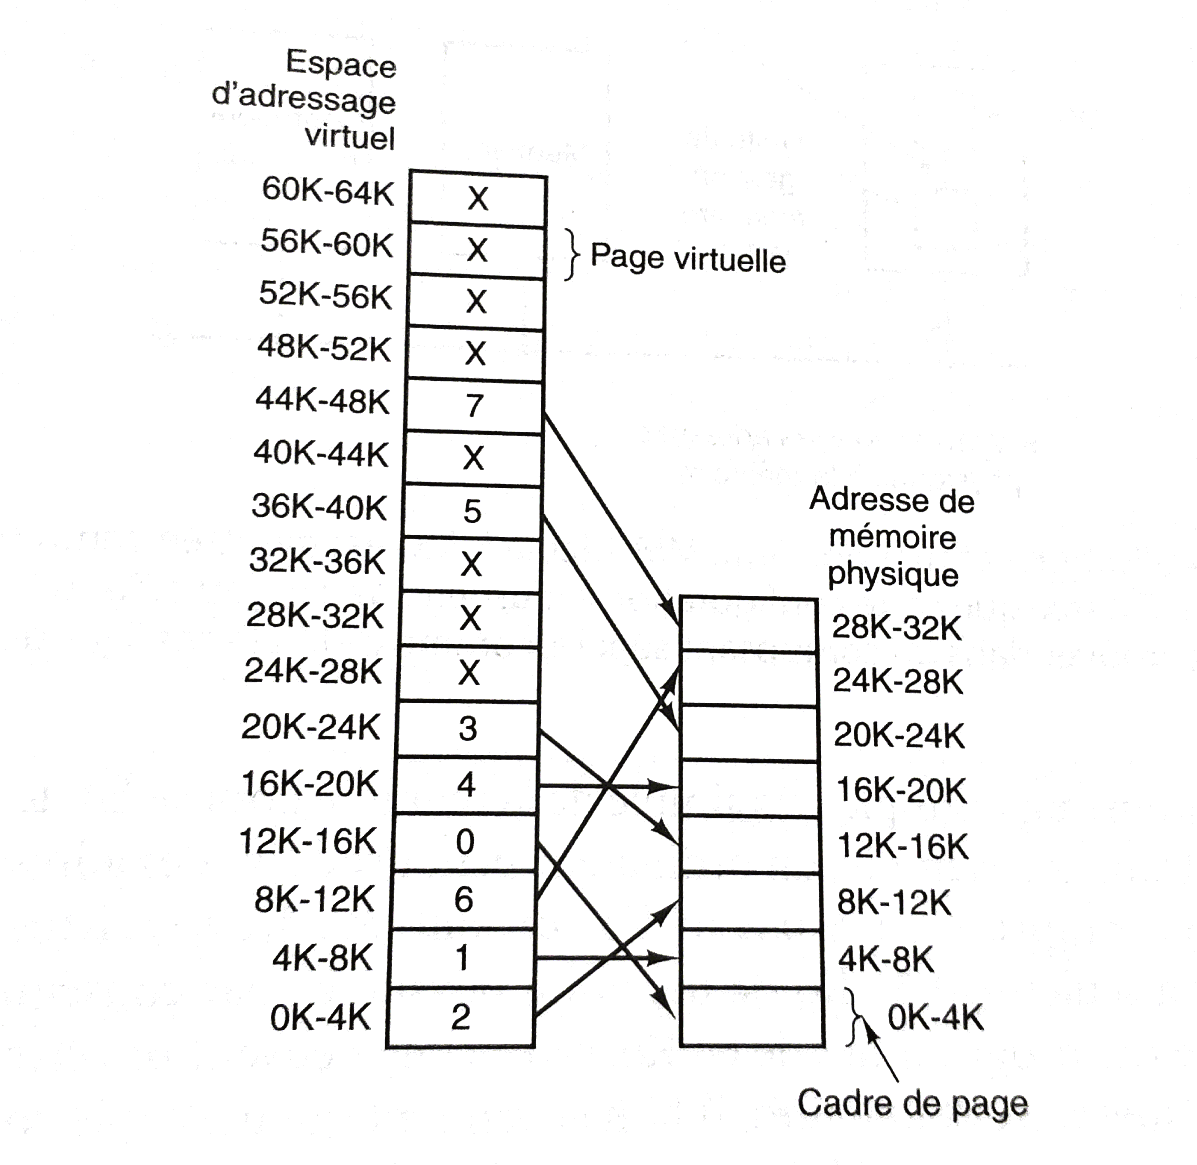
\includegraphics[width=5cm]{images/memory_page_frame.png}
    \caption{\label{pic:memory_page_frame} Correspondance entre les adresse virtuelles, stockées dans des pages, et les adresses physiques, stockées dans des cadres de pages.  \cite{tanenbaum2008systeme})}.
\end{figure}


\subsubsection{La taille des pages}
%%%%%%%%%%%%%%%%%%%%%%%%%%%%%%%%%%%
Les transferts de données entre la mémoire et le stockage se font par page. Ainsi une page ne peut se trouver à la fois en mémoire et sur le disque. En fonction des applications et de l'algorithme de remplacement de pages (voir \autoref{sec:deplacement_page}) ces transferts peuvent être fréquents. Le choix de la taille de page doit alors être pris en considération pour obtenir les performances de l'application attendus.
Plus la taille des pages est petite, plus l'utilisation effective de la mémoire sera proche de la quantité mémoire disponible. Avec de grandes pages, les processus n'en utilisant qu'une faible partie, réduise la mémoire disponible pour les autres processus. Si les \textit{défauts de pages} sont fréquent, la quantité de mémoire à déplacer entre la mémoire et le stockage et d'autant plus grande.

Aujourd'hui, les systèmes d'exploitation utilisent des page mesurant $4 KiB$. Cette taille est un bon compromis entre la gestion complexe de la table des pages qui doit être parcouru le moins souvent possible, et la meilleure gestion de la mémoire possible. 
Cependant, les systèmes d'exploitation récents permettent d'utiliser des tailles de pages plus grandes pour certaines applications qui pourraient en bénéficier. Ces grandes pages ou \textit{large pages} ou \textit{huge pages}, sont des pages de taille allant de 2 MiB à plusieurs GiB et peuvent être allouées de deux façons. La première est transparente pour l'utilisation. C'est le système d'exploitation qui analyse les accès et \textit{comprend} que le jeux de données accédé est grand et que l'application pourrait profiter de l'utilisation de grande page. Ce mécanisme est appelé \textit{`Transparent Huge Pages} (THP) car il est géré automatiquement par le système \cite{LinuxTHP2019}. Le deuxième façon pour utiliser des grandes pages est d'allouer la mémoire manuellement dans le code. Un exemple d'allocation est donnée dans le code du noyau Linux \cite{LinuxHUGE2019}.

Avec des pages larges, la TLB (voir \autoref{sec:tlb}) est plus rapide à parcourir, sa latence est donc réduite. De plus, leur utilisation vise à réduire le nombre de \textit{faute de page}, les pages couvrant un espace d'adressage plus large. De plus, les pages étant plus grand, les cadres de pages correspondant le sont aussi: les adresses mémoires sont contiguës sur un plus grand intervalle d'adresse. Cela peut avoir pour effet de réduire les conflits d'associativité dans les caches. Notamment pour des tailles de cache proche de de la taille d'une ligne de cache \cite{LinuxHUGETEST2019}.






%%%%%%%%%%%%%%%%%%%%%%%%%%%%%%%%%%%%%%%%%%%%%%%%%%%%%%%%%%%%%%%%%%%
\subsection{Memory Management Unit (MMU)} \label{sec:mmu}
%%%%%%%%%%%%%%%%%%%%%%%%%%%%%%%%%%%%%%%%%%%%%%%%%%%%%%%%%%%%%%%%%%%
La \textit{MMU} est un composant matériel responsable de la gestion de la mémoire paginée. Il est, depuis le processeur 80386 d'Intel, intégré directement au processeur. Les missions de la MMU sont multiples. Il est responsable de la traduction des adresses virtuelles en adresse physique. Lorsque le processeur réalise un accès mémoire, il n'envoie pas directement l'adresse sur le bus mémoire. Cette adresse (virtuelle) est d'abord traduite (en adresse physique) par la MMU qui s'occupe de l'écrire sur le bus mémoire. La \textit{MMU} doit aussi s'occuper de déplacements des pages entre la mémoire et le disque quand c'est nécessaire (défaut de page). Elle est aussi responsable de sécuriser les accès et d'empêcher un programme d'écrire dans une page qui ne lui appartient pas. Il peut alors lever une exception (\textit{SIGSEGV}) pour interrompre le programme. 

\subsubsection{Table des pages} \label{sec:table_page}
%%%%%%%%%%%%%%%%%%%%%%%%%%%%%%%%%%%
La table des pages à pour fonction de faire correspondre les pages virtuelles (\textit{Virtual Page Number} (\textit{VPN})) à leur cadre de page correspondant (\textit{Physical Page Number} (\textit{PPN}) représenté par les flèches de la \autoref{pic:memory_page_frame}. C'est grâce à cette table que les adresses virtuelles peuvent être traduites. L'adresse de cette table est stockée dans un registre (\textit{Page Table Base Register} (\textit{PTBR}). Une fois la traduction de l'adresse virtuelle de la page réalisée, les bits de décalage \textit{Virtual Page Offset} (VPO) sont utilisée pour sélectionner la donnée voulue dans cette page. La \autoref{fig:memory_page_table_nbits} montre un exemple du fonctionnement de la table des pages pour la traduction d'une adresse virtuelle. Dans la table des pages est stockés le numéro du cadre de page, utilisé pour la construction de l'adresse physique. Cette entrée contient également d'autres informations (\autoref{pic:memory_page_table_entry}) comme les droits d'accès à la page ou si elle a été modifiée (pour la gestion de cohérence).

\begin{figure}
    \centering
    \begin{subfigure}[b]{\linewidth}\centering
        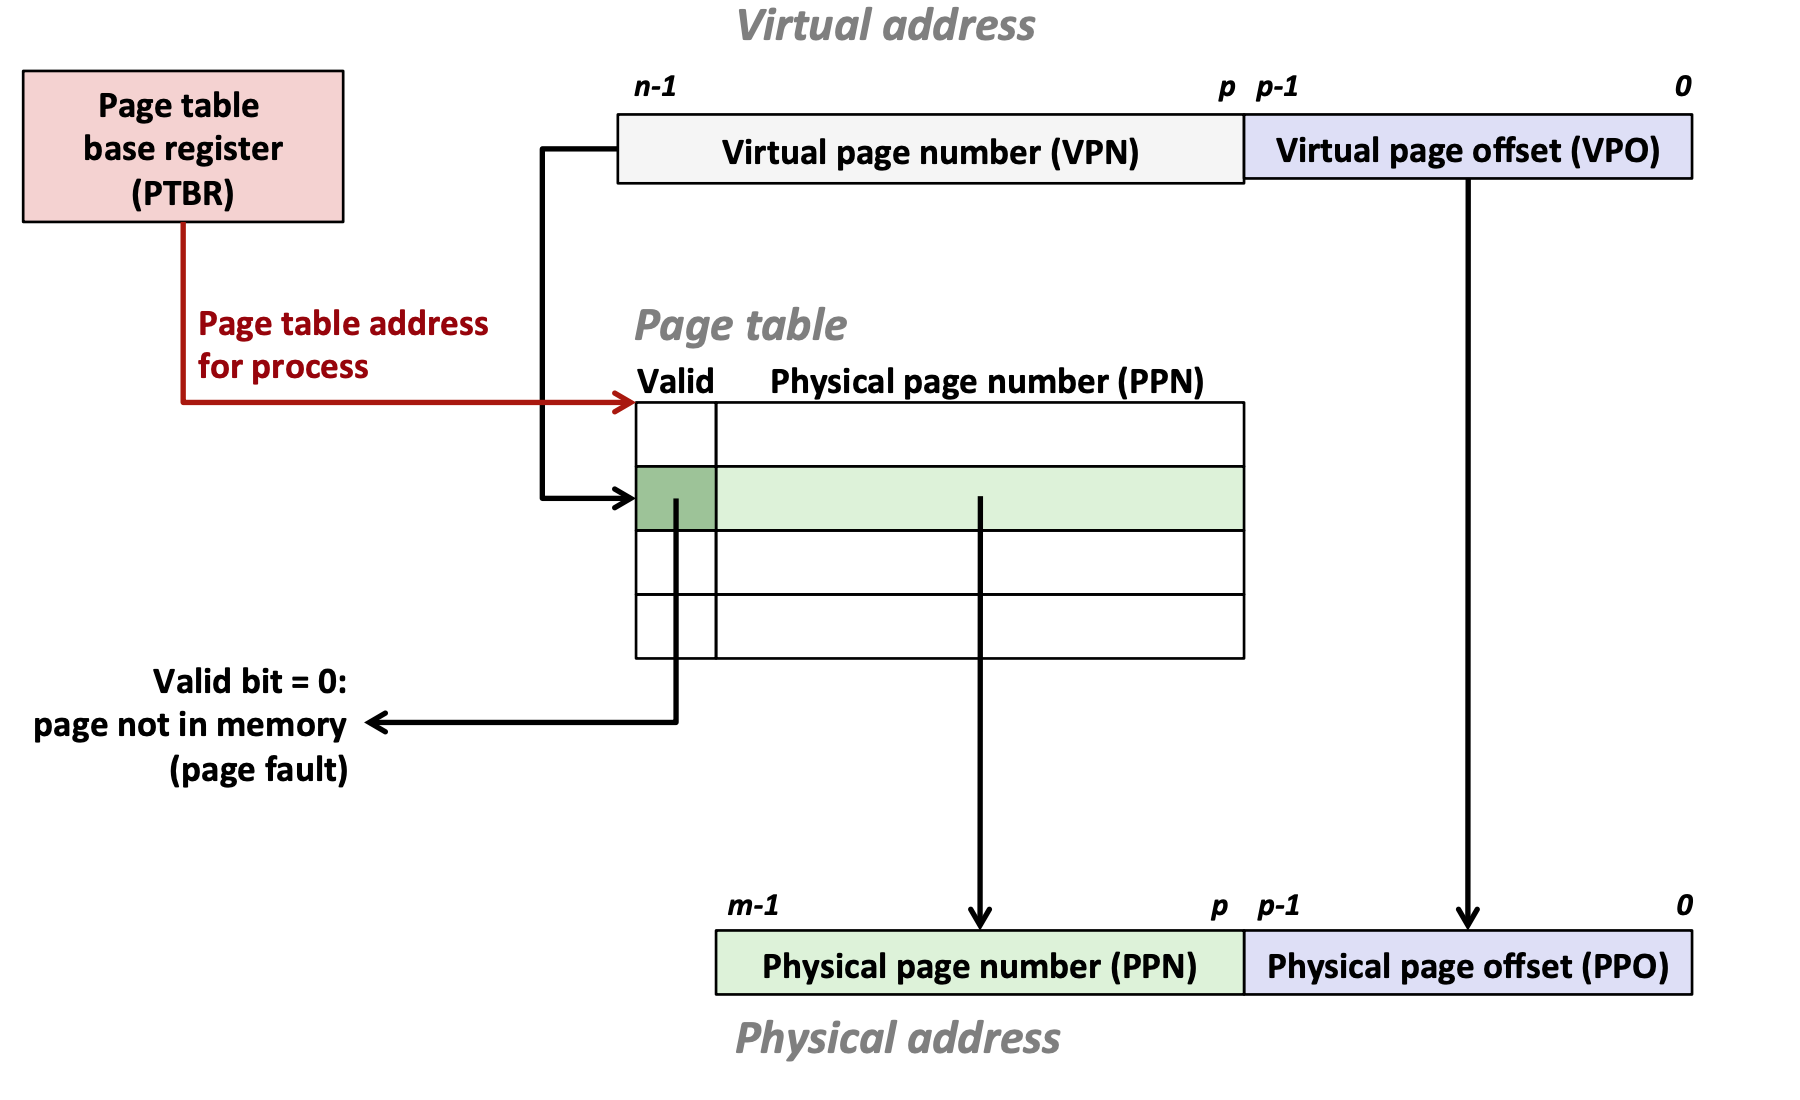
\includegraphics[width=0.7\linewidth]{images/memory_page_table_nbits.png}
        \caption{L'adresse physique de la table des pages est stockée dans un registre (\textit{PTBR}). La MMU utilise une partie des bits de l'adresse virtuelle (\textit{VPN}) pour trouver la ligne correspondant à la page dans cette table. A cette entrée de la table est stockée l'adresse du cadre de page correspondant à la page virtuelle (\textit{PPN}). L'adresse \textit{PPN} associée aux bits restant de l'adresse virtuelle (\textit{VPO}) permet de construire l'adresse physique de la donnée voulue \cite{Mowry2012}.}
        \label{pic:memory_page_table_nbits}
    \end{subfigure}
    ~ %add desired spacing between images, e. g. ~, \quad, \qquad, \hfill etc. 
      %(or a blank line to force the subfigure onto a new line)
    \begin{subfigure}[b]{\linewidth}\centering
        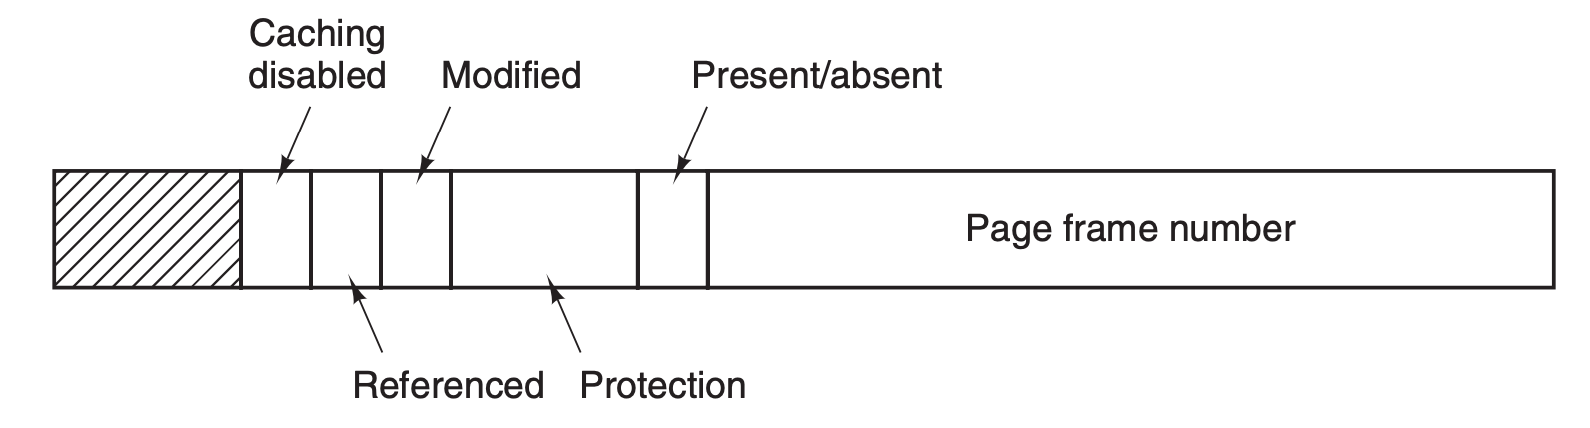
\includegraphics[width=0.7\linewidth]{images/memory_page_table_entry.png}
        \caption{Pour le fonctionnement de la MMU, la table des pages conserve plusieurs informations importantes pour chaque entrée de page, en plus de l'adresse du cadre de page. Un bit de présence permet de savoir si la page est en mémoire, ou sur le disque. La protection assure qu'un utilisateur ne puisse pas modifier des données de lui appartenant pas. Un bit de modification est utilisé pour la cohérence \cite{tanenbaum2008systemes}.}
        \label{pic:memory_page_table_entry}
    \end{subfigure}
    

    \caption{Exemple de fonctionnement de la MMU pour la traduction d'une adresse virtuelle en utilisant une table de page à un seul niveau.). }\label{fig:memory_page_table_un_niveau}
\end{figure}


Cependant, la table des pages peut rapidement prendre beaucoup de places et son stockage en mémoire peut affecter les performances des programmes. Par exemple, un machine utilisant des adresses de 32 bits aura une table de page mesurant plus de 16 MiB, et chaque processus possède sa propre table. De plus, pour des pages de 4 KiB et un espace d'adressage de 32 bits utilise 1 million de page. Le parcours de la table peut être long, d'autant que les architecture modernes utilisent des adresses de 64 bits. Pour répondre à ce challenge, les architectes ont implémentés deux techniques permettant d'accélérer la traduction. La première est d'utiliser un cache qui stocke les traductions récentes et évite la traduction permanente des adresses virtuelles. La deuxième est de modifier la structure de la table de pages en implémentant une table à plusieurs niveaux grâce à une structure d'arbre. 


\paragraph{Accélérer le parcours de la table grâce à une table multiniveaux} Le parcours de la table de page est primordiale car une seule instruction peut nécessiter de la parcourir 3 fois avant d'être exécuté (adresse de l'instruction, et adresses des deux opérandes). La \autoref{pic:memory_page_table_multi} montre un table utilisant 4 niveaux. Le premier niveau est appelé répertoire des pages (\textit{Page Directory}). La MMU partage l'adresse virtuelle de la page (\textit{VPN}) en $k$ morceaux permettant de parcourir les $k$ niveau de la table de pages. Les derniers bits sont utilisés pour le décalage dans la page mémoire et la construction de l'adresse physique. Ainsi les différentes pages  n'ont pas besoin d'être stocké continuellement en mémoire. Seul le répertoire des pages, entrée commune à toutes les pages, est conservé en mémoire. 


\begin{figure}
    \center
    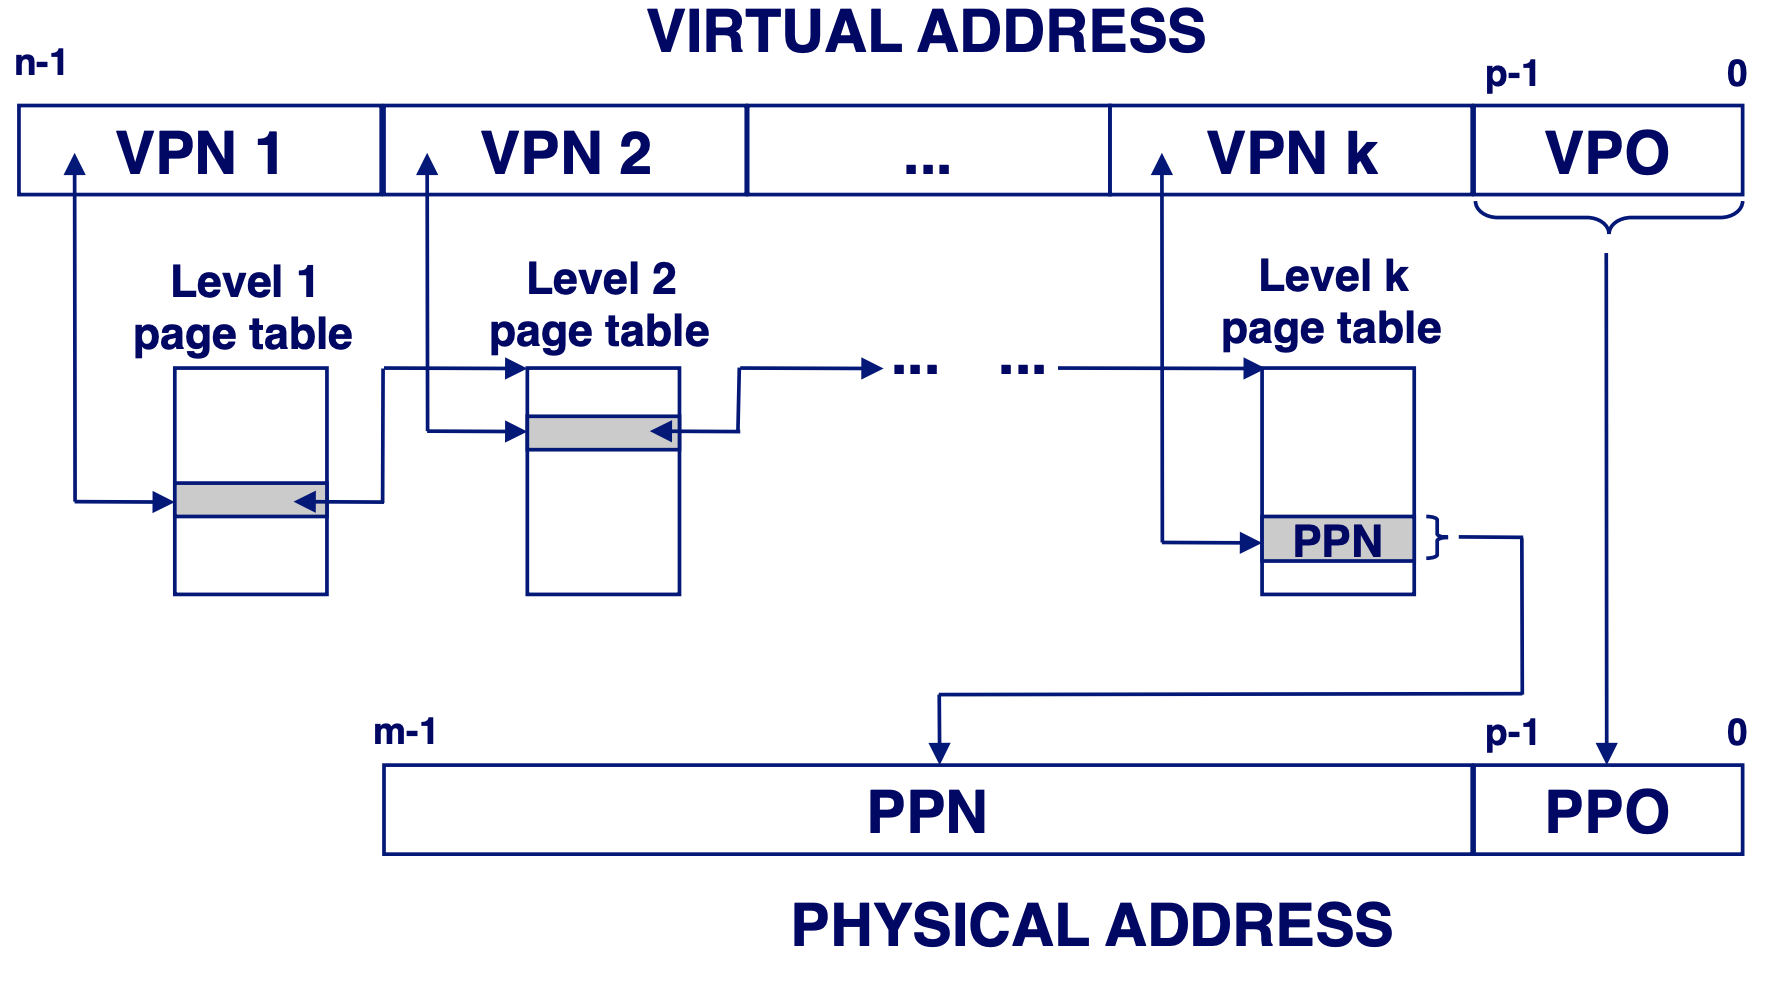
\includegraphics[width=10cm]{images/memory_page_table_multi2.png}
    \caption{\label{pic:memory_page_table_multi} Exemple d'utilisation d'une table de pages à \textit{k} niveaux \cite{Mowry2012}. L'adresse virtuelle est découpé en $k+1$ morceaux. Le premier morceau (\textit{VPN 1}) détermine la ligne dans la premier table (située à l'adresse \textit{PTBR}). Cette entrée permet d'obtenir l'adresse physique de la page de niveau 2. L'entrée dans cette page est déterminée à partir du second morceau (\textit{VPN 2}). Ce même procédé est utilisé pour parcourir tous les niveaux table. Dans la dernière table (\textit{VPN k}) est stockée l'adresse physique de la page ciblée (\textit{PPN}). L'adresse physique est construite à partir de cette adress \textit{PPN} et du décalage \textit{VPO} (derniers bits de l'adresse virtuelle).  }.
\end{figure}



\paragraph{Le cache de traduction: Translation Lookaside Buffer.} \label{sec:tlb}
Les pages étant de plus en plus grandes (4 KiB sur les architectures actuelles), les processus font généralement beaucoup d'accès à des adresses appartenant à un nombre de pages réduits. Cette observation est à l'origine de la création d'un cache \textbf{TLB} conservant les traductions de pages récentes. Ce dispositif matériel est généralement disposé dans la MMU. Dans ce cache sont généralement stockés: l'adresse de la page et du cadre de  page correspondant, les droits et protections, la validité ainsi qu'un bit de modification (\textit{dirty bit}). 
La \autoref{pic_memory_page_table_tlb} résumer comment le TLB est utilisé par la MMU lors de la traduction d'une adresse virtuelle. Deux cas sont possibles: la page est présente dans le TLB (évènement \textit{TLB-hit}, \autoref{pic_memory_page_table_tlb_hit}), ou elle ne l'est pas (évènement \textit{TLB-miss}, \autoref{pic_memory_page_table_tlb_miss}).


\begin{figure}
    %\centering
    \begin{subfigure}[t]{0.48\linewidth}\centering
        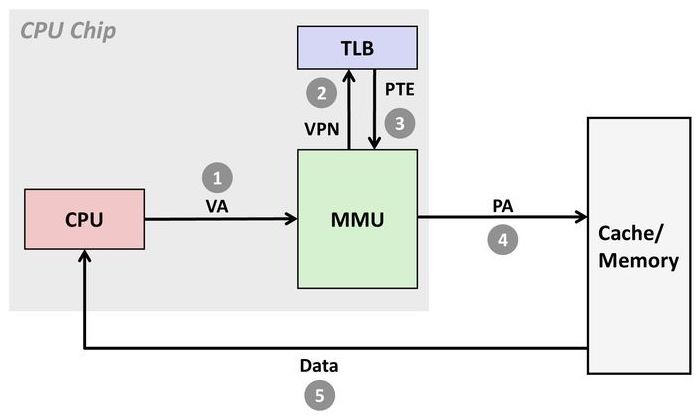
\includegraphics[width=\linewidth]{images/memory_page_table_tlb_hit.jpg}
        \caption{Si la traduction de la page se trouve dans la TLB, elle renvoie le pointeur vers l'entrée de la page (PTE) directement à la MMU (étape 3) qui peut alors réaliser la traduction de l'adresse virtuelle. Elle accède ensuite directement à la donnée voulue en mémoire grâce à l'adresse physique traduite \textit{PA} (étape 4)}
        \label{pic_memory_page_table_tlb_hit}
    \end{subfigure}
    ~ %add desired spacing between images, e. g. ~, \quad, \qquad, \hfill etc. 
      %(or a blank line to force the subfigure onto a new line)
    \begin{subfigure}[t]{0.48\linewidth}\centering
        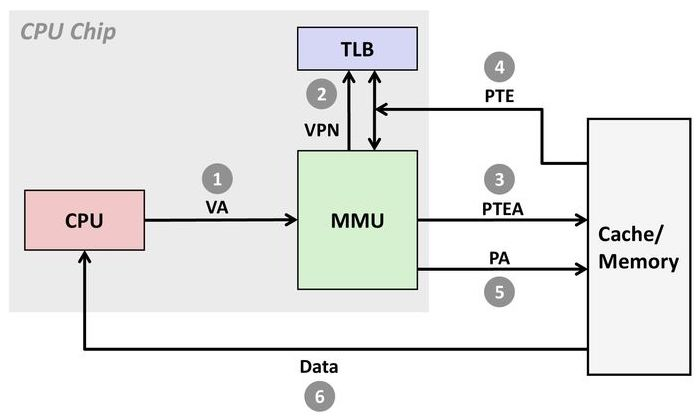
\includegraphics[width=\linewidth]{images/memory_page_table_tlb_miss.jpg}
        \caption{Si la page ne se trouve pas dans la TLB, la MMU doit s'occuper de la traduction  de PTE. Elle utilise sa table des pages (multiniveaux par exemple) pour trouver l'adresse physique \textit{PTEA} où est stockée l'adresse de l'entrée de la page \textit{PTE} (étape 3). La traduction est copiée dans la TLB pour éviter une nouvelle traduction (étape 5). Enfin, elle peut réaliser la traduction de l'adresse virtuelle en adresse physique (étape 5)}
        \label{pic_memory_page_table_tlb_miss}
    \end{subfigure}
    \caption{Fonctionnement de la TLB. Lors d'un accès mémoire le processeur envoie l'adresse virtuelle \textit{VA} à la MMU pour la traduire (étape 1). La MMU vérifie si la traduction \textit{VPN} a été faite récemment et si l'adresse physique a été sauvée dans la TLB (étape 2) \cite{Mowry2012}.
    \label{pic_memory_page_table_tlb}}
\end{figure}




Pour une architecture récente telle que Skylake, le cache de traduction est composé de trois caches répartis en deux niveau. Deux caches de niveau 1 se partagent les adresses d'instructions (\textit{ITLB}) et de données (\textit{DTLB}) et possèdent des entrées pour les différentes taille de pages (4 KiB, 2 MiB, 4 MiB, 1 GiB). Le niveau 2 unifie les deux caches de niveau 1 grâce un cache utilisant 12 sets  (\textit{12-way set associative}) et 1536 entrée \cite{Wikichipb}.




\subsubsection{Déplacement de page} \label{sec:deplacement_page}
%%%%%%%%%%%%%%%%%%%%%%%%%%%%%%%%%%%
Lorsque la demande mémoire est supérieur à l'espace disponible, la totalité des processus ne peut pas y être stocké. Ainsi, la totalité des pages allouées ne se trouvent pas toute en mémoire à un instant donné. Pour cela, la MMU tient une liste des pages se trouvant en mémoire en utilisant pour chaque page un bit de présence/absence. Dans l'exemple de la \autoref{pic:memory_page_frame}, si un processus à accède à l'adresse $33000$, sa table des pages et constate que la page n'est pas présente en mémoire. Cet évènement est appelé un \textbf{défaut de page} (\textit{page fault}). La système doit alors déplacer une page de la mémoire vers le stockage pour faire de la place pour cette nouvelle page. Le choix de la page à déplacer se fait grâce à un algorithme de remplacement de page. De la même façon que pour la gestion des lignes de cache, il faut une méthode efficace de remplacement pour éviter de remplacer une page qui sera accédée par l'instruction suivante. Plusieurs algorithmes existent: First In First Out (FIFO) remplace la page la plus vieille, Not Recently Used (NRU) remplace la page non utilisée depuis longtemps, Seconde Chance implémente l'algorithme FIFO mais cherche en priorité une page non-référencée. Pour des applications réalisant des accès mémoire sur plusieurs pages, l'algorithme choisi peut avoir un fort impacte sur sa performance.



te